An axis aligned rectangle classifier is a classifier than assigns the value 1 to a point if and only if it is inside a certain rectangle. Formally, given real numbers $a_1\le b_1, a_2 \le b_2$, define the classifier $f_{(a_1,b_1,a_2,b_2)}$ on an input $\x$ with coordinates $(x_1,x_2)$ by
    \[ 
    f_{(a_1,b_1,a_2,b_2)}(x_1, x_2) =
    \begin{cases} 
      1 & \text{if } a_1\le x_1\le b_1 \text{ and }  a_2\le x_2\le b_2\\
      -1 & \text{otherwise}.
   \end{cases}
\]
The function class of all axis-aligned rectangles in the plane is defined as
\begin{align*}
    \mathcal{F}_{\text{rec}}^2 = \{ f_{(a_1,b_1,a_2,b_2)}(x_1, x_2): a_1 \le b_1, a_2 \le b_2\}.
\end{align*}
We will assume that the true labels $y$ of the data points $(\x,y)$ are given by some axis-aligned rectangle (this is the realizability assumption discussed in class). The goal of this question is to come up with an algorithm which gets small classification error with respect to any distribution $D$ over $(\x,y)$ with good probability.

The loss function we use throughout the question is the 0-1 loss. It will be convenient to denote a rectangle marked by corners $(a_1,b_1,a_2, b_2)$ as $B(a_1,b_1,a_2, b_2)$. Let $B^*=B(a_1^*, b_1^*, a_2^*, b_2^*)$ be the rectangle corresponding to the function $f_{(a_1^*, b_1^*, a_2^*, b_2^*)}$ which labels the datapoints (meaning that for all $(\x,y)$ drawn from distribution $D$, $f_{(a_1^*, b_1^*, a_2^*, b_2^*)}(\x)=y$). Let $S=\{(\x_i,y_i), i \in [n]\}$ be a training set of $n$ samples drawn i.i.d. from $D$. 
Please see Fig.~\ref{fig:rect} for an example.\\

\begin{figure}[h]
    \centering
    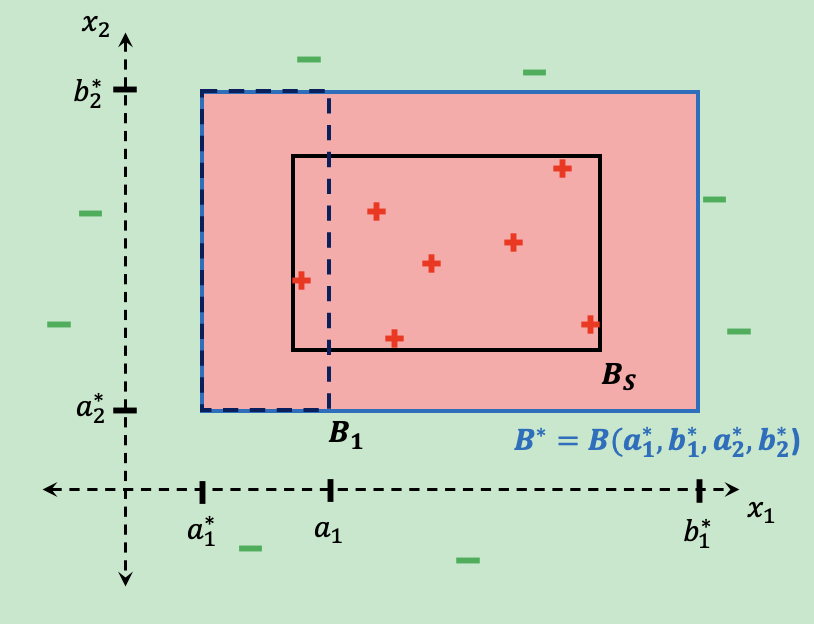
\includegraphics[width=0.5\textwidth]{rect.png}
    \caption{Learning axis-aligned rectangles in two dimensions, here $+$ (red) denotes datapoints in training set $S$ with label 1 and $-$ (green) denotes datapoints with label -1. The true labels are given by rectangle $B^*$ (solid blue line), with everything outside $B^*$ being labelled negative and inside being labelled positive. $B_S$ (solid black line) is the rectangle learned by the algorithm in \textbf{2.2}. $B_1$ (dashed black line) is defined in \textbf{2.3}.}
    \label{fig:rect}
\end{figure}


\textbf{2.1} (\blue{4pts}) We will follow the general supervised learning framework from class. For a function $f_{(a_1,b_1,a_2,b_2)}$, define the empirical risk with respect to 0-1 loss as $\widehat{\mathcal{R}}(f_{(a_1,b_1,a_2,b_2)})=\sum_{i=1}^n\mathbb{I}\{f_{(a_1,b_1,a_2,b_2)}(\x_i)\neq y_i\}$. Given the 0-1 loss, and the function class of axis-aligned rectangles, we want to find an empirical risk minimizer. Consider the algorithm which returns the smallest rectangle enclosing all positive examples in the training set. Prove that this algorithm is an empirical risk minimizer, meaning that it minimize $\widehat{\mathcal{R}}(f)$ over all $f$ in $\mathcal{F}_{\text{rec}}^2$. (\emph{Hint: use the realizability assumption.})\\

\noindent{\fontsize{11}{12}\selectfont\textbf{Solution 2.1}}

Since the algorithm returns the \textbf{smallest} rectangle enclosing all positive examples, we suppose it as $B_S$.

By the definition of realizability assumption, $B^*$ in the description of Figure 1, we know that everything outside $B^*$ being labeled negative and inside being labeled positive.

Therefore, we have:
\[
B_S \subseteq B^*
\]
\textbf{Proof of claim.} \\
Define $S_+$ as the set of all positive examples:
\[
S_+ = \{\mathbf{x}_i \in S, y_i = 1\}
\]
By realizability, for all $x_i \in S_+$, we have $x_i \in B^*$. 
Since $B_S$ is defined as the \emph{smallest} axis-aligned rectangle that encloses
all points in $S_+$, ie. $B_S \subseteq S_+$ \;, and $B^*$ is an axis-aligned rectangle that also encloses all
points in $S_+$, it follows that $B_S \subseteq B^*$.

\medskip
\textbf{Thus},
\[
\forall \mathbf{x}_i \in S_+ , \mathbf{x}_i \in B_S ,
\]

which means for all $\mathbf{x}_i$, 
\[
f_{B_S}(\mathbf{x}_i) = 1
\]

Define:
\[
S_- = \{\mathbf{x}_j \in S, y_j = -1\}
\]

Since
\[
\mathbf{x}_j \notin B^*
\]

Therefore, by define
\[
x_j \notin B_S
\]
\[
\textbf{and if}
\]
\[
f_{B_S}(\mathbf{x}_j) = -1
\]

Hence, the empirical risk satisfies
\[
\hat{R}(f_{B_S}(\mathbf{x})) = \sum_{i=1}^n \mathbb{I}\{f_{B_S}(\mathbf{x_i}) \neq y_i\} = 0,
\]

Since the empirical risk is always non-negative for any hypothesis. where our $\hat{R}(f_{B_S})$ shown that the empirical risk equals zero, this shows that $f_{B_S}$ minimizes the empirical risk over all $f \in \mathcal{F}_{\text{rec}}^2$.
Therefore, the algorithm is an empirical risk minimizer.
\bigskip

\textbf{2.2} (\blue{4pts}) Our next task is to show that the algorithm from the previous part not only does well on the training data, but also gets small classification error with respect to the distribution $D$.  Let $B_S$ be the rectangle returned by the algorithm in \textbf{2.1} on training set $S$, and let $f_S^{ERM}$ be the corresponding hypothesis. First, we will convince ourselves that generalization is inherently a probabilistic statement. Let a \emph{bad} training set $S'$ be a training set such that $R(f_{S'}^{ERM})\ge 0.5$. Pick some simple distribution $D$ and ground-truth rectangle $B^*$, and give a short explanation for why there is a \emph{non-zero} probability of seeing a bad training set.\\

\noindent{\fontsize{11}{12}\selectfont\textbf{Solution 2.2}}

Let us pick a simple discrete distribution $D$ supported on four points
$D = \{x_1, x_2, x_3, x_4\}$, where $x_1, x_2, x_3$ lie inside the ground-truth
rectangle $B^*$ and have label $+1$, and $x_4$ lies outside $B^*$ and has label $-1$.
Assume $D$ is the uniform distribution over these four points, so that
$P(x_i)=0.25$ for all $i$.\\

Consider a training set $S'$ of size $1$. With probability 

\[
P(\mathbf{x}_i) = 0.25
\] 

we have
$S' = \{x_1\}$. In this case, the algorithm in 2.1 returns the smallest rectangle
$B_{S'}$ containing $x_1$, which is a very small rectangle that does not contain
$x_2$ or $x_3$.

If $S'$ only contains $\{\mathbf{x}_1\}$, then the algorithm in \textbf{2.1} returns a tiny rectangle $B_{S'}$ that only covers $\mathbf{x}_1$. And $B_{S'}$ will misclassify $\mathbf{x}_2$ and $\mathbf{x}_3$ as negative.

Then
\[
R(f_{S'}^{ERM}) = P(\mathbf{x}_2) + P(\mathbf{x}_3) = 0.25 + 0.25 = 0.5.
\]

Since the event $S' = \{x_1\}$ occurs with non-zero probability, this shows that
there is a non-zero probability of observing a bad training set. This demonstrates
that generalization is inherently a probabilistic statement.
\bigskip

\textbf{2.3} (\blue{8pts})  Though there is non-zero probability seeing bad training set, we will now show that \emph{with high probability} over the training dataset $S$, $f_S^{ERM}$ \emph{does} get small error. Show that if $n\ge \frac{4 \log (4/\delta)}{\epsilon}$ then with probability at least $1-\delta$, $R(f_S^{ERM})\le \epsilon$.
    
    To prove this follow the following steps. Let $a_1 \ge a_1^*$ be such that the probability mass (with respect to $D$) of the rectangle $B_1=B(a_1^*, a_1, a_2^*, b_2^*)$ is exactly $\epsilon/4$. Similarly, let $b_1\leq b_1^*, a_2\geq a_2^*,b_2\leq b_2^*$ be numbers such that the probability mass (with respect to $D$) of the rectangles $B_2=B(b_1,b_1^*, a_2^*, b_2^*), B_3=B(a_1^*, b_1^*, a_2^*, a_2), B_4=B(a_1^*, b_1^*, b_2, b_2^*)$ are all exactly $\epsilon/4$.
    \begin{itemize}
        \item Show that $B_S \subseteq B^*$.
        \item Show that if $S$ contains (positive) examples in all of the rectangles $B_1, B_2, B_3, B_4$ then $R(f_S^{ERM})\le \epsilon$. (Hint: think about the geometric relationship between $B_i$ and $B_S$, $i\in\{1,2,3,4\}$)
        \item For each $i \in \{1,\dots, 4\}$ upper bound the probability that $S$ does not contain an example from $B_i$.
        \item Use the union bound to conclude the argument.
    \end{itemize}

\noindent{\fontsize{11}{12}\selectfont\textbf{Solution 2.3}}

According to 2.1, We have:
\[
B_S \subseteq B^*
\]

If $S$ contains (positive) examples in all of $B_1, B_2, B_3, B_4$, and we define them as four strips along the edges of $B^*$, So we have:
\[
B_1, B_2, B_3, B_4 \subseteq B^*
\]
\[
\mathbb{P}_D(B_i) = \frac{\epsilon}{4}, \quad i=1,2,3,4.
\]

Suppose that the training set S contains at least one positive example in each $B_i$. Then ERM must expand its rectangle to include these points, so
\[
B^*-B_S \subseteq \bigcup_{i=1}^4 B_i.
\]

\[
R(f_S^{\mathrm{ERM}}) = \mathbb{P}_D(B^* - B_S) \le \sum_{i=1}^4 \mathbb{P}_D(B_i) = \epsilon.
\]

For any $B_i$, the probability that it contains no postive examples is: $1 - \frac{\epsilon}{4}$

So using the inequality:
\[
1-x \le e^{-x}
\]

We have 

\[
\left(1 - \frac{\epsilon}{4}\right)^n \le e^{-n \epsilon /4},
\]

Define the bad event E as "at least one strip contains no sample":
\[
E = \bigcup_{i=1}^4 \{\text{no sample falls in } B_i\}.
\]

By the union bound,

\[
\mathbb{P}(E) \le \sum_{i=1}^4 e^{-n \epsilon /4} = 4 e^{-n \epsilon /4}.
\]

To ensure $\mathbb{P}(E) \le \delta$, we get
\[
4 e^{-n \epsilon /4} \le \delta \quad 
\]

\[
\quad n \ge \frac{4 \log(4/\delta)}{\epsilon}.
\]

Therefore,  if the number of training samples satisfies 
\[
\quad n \ge \frac{4 \log(4/\delta)}{\epsilon}.
\]

Then with probability at least $1- \delta$, each of the four strips $B_i$ contains at least one training point. The ERM rectangle $B_S$ satisfies 
\[
R(f_S^{\mathrm{ERM}}) \le \epsilon.
\]

\bigskip

\textbf{(Bonus) 2.4} (\blue{8pts}) Repeat the previous question for the function class of axis-aligned rectangles in $\R^d$. Specifically, the current function class is $\mathcal{F}_{\text{d-rec}}=\{f_{(a_1,b_1,a_2,b_2,\dots,a_d,b_d)}(x_1,x_2,\dots,x_d):a_i\leq b_i, i\in\{1,2,\dots,d\}\}$ and a datapoint $\x\in\R^d$ is predicted to be $1$ by $f_{(a_1,b_1,a_2,b_2,\dots,a_d,b_d)}(x_1,x_2,\dots,x_d)$ if $a_i\leq x_i\leq b_i$ for all $i\in\{1,2,\dots,d\}$ and $-1$ otherwise. We will still assume realizability. To show this, try to generalize all the steps in the above question to higher dimensions, and find the number of training samples $n$ required to guarantee that $R(f_S^{ERM})\le \epsilon$ with probability at least $1-\delta$. \\

\noindent{\fontsize{11}{12}\selectfont\textbf{Solution 2.4}}

Similar to 2.1, by definition:  $f_{(a_1,b_1,a_2,b_2,\dots,a_d,b_d)}(x_1,x_2,\dots,x_d)$ if $a_i\leq x_i\leq b_i$ for all $i\in\{1,2,\dots,d\}$
the algorithm returns the smallest hyper-rectangle enclosing all positive examples in $\mathbb{R}^d$,
we denote it by $B_S$. And according to Realizability assumption, we have target set, $B^*$ in $\mathbb{R}^d$, that all positive examples lie inside $B^*$ and all negative examples lie outside $B^*$. 
\bigskip
Comparing the coordinates dimensionally, esaily We have:
\[
B_S \subseteq B^* \;
\] 
As in the two-dimensional case, the algorithm achieves zero empirical risk under
the realizability assumption. We now bound the true risk.
For each dimension $i=1,\dots,d$, consider the two boundary regions (small fractions)
adjacent to the faces $x_i=a_i^*$ and $x_i=b_i^*$ of $B^*$. We choose these $2d$ fractions such that each fraction has probability mass at most
$\varepsilon/(2d)$ under some distribution $D$.(similar to 2.3)

\medskip
If the training set contains at least one positive example in each of the $2d$ fractions, then the learned rectangle $B_S$ must contain the remaining central region of $B^*$, and any misclassified point must lie in one of the fractions.
Thereby, in this case,
\[
R(f_S^{ERM}) \le 2d \cdot \frac{\varepsilon}{2d} = \varepsilon.
\]

For any fixed fraction, the probability that none of the $n$ i.i.d.\ training samples
falls inside it is at most $(1-\varepsilon/(2d))^n$ and it is$\le\delta$.
By a union bound over all $2d$ fractions, the probability that at least one fraction
contains no training sample is at most
\[
2d \left(1-\frac{\varepsilon}{2d}\right)^n  \le
2d \; e^{-\frac{n\varepsilon}{2d}} \le
\delta
\]
To ensure this probability is at most $\delta$, we can choose loose up-bound $\delta$
\begin{align*}
2d \; e^{-\frac{n\varepsilon}{2d}} &\le \delta \\
e^{-\frac{n\varepsilon}{2d}} &\le {\delta \over{2d}} \\
-\frac{n\varepsilon}{2d} &\le \ln{{\delta \over{2d}}}\\
\frac{n\varepsilon}{2d} &\ge  \ln{{2d \over{\delta}}}\\
n &\ge \frac{2d}{\varepsilon}\ln\frac{2d}{\delta}
\end{align*}

Which means,
\[
n \ge \frac{2d}{\varepsilon}\ln\frac{2d}{\delta} \quad  \textbf{has} \: \Pr(R(f_S^{\mathrm{ERM}}) > \varepsilon) \le \delta
\]
By whole probability rule,
\[
\Pr(R(f_S^{\mathrm{ERM}}) \le \varepsilon) = 1 - \Pr(R(f_S^{\mathrm{ERM}}) > \varepsilon)
\]

Hence, with probability at least $1-\delta$, the learned hypothesis satisfies
$R(f_S^{ERM}) \le \varepsilon$.
\[
\Pr(R(f_S^{\mathrm{ERM}}) \le \varepsilon) \ge 1- \delta 
\]

\bigskip

\bigskip